\documentclass[10pt]{beamer}

\usetheme[progressbar=frametitle]{metropolis}
\usepackage{appendixnumberbeamer}
\usepackage[english,spanish]{babel}
\usepackage{relsize}
% \usepackage[utf8]{inputenc} % Required for inputting international characters
% \usepackage[T1]{fontenc} % Output font encoding for international characters

\usepackage{booktabs}
\usepackage{bm}
\usefonttheme{professionalfonts}
\usepackage{mathspec}
\usepackage{todonotes}
\usepackage[scale=2]{ccicons}

\usepackage{pgfplots}
\usepgfplotslibrary{dateplot}

\usepackage{xspace}
\newcommand{\themename}{\textbf{\textsc{metropolis}}\xspace}

\title{Advanced Natural Language Processing Techniques to Profile Cybercriminals}
\subtitle{\textsc{Proyecto de grado 1}}
\date{\today}
% \date{}
\institute{Escuela Colombiana de Ingenier\'{\i}a Julio Garavito}
\titlegraphic{\hfill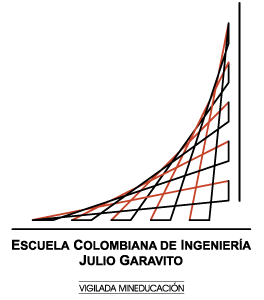
\includegraphics[height=1.5cm]{Images/escuela-logo.png}}

% 1.Nombre del proyecto
% 1.Integrantes
% 1.Director
% 2.Agenda
% 3.Objetivo general y específicos (para todo el proyecto: PGR1 y PGR2)
% 4.Justificación del proyecto
% 5.Resultados propuestos
% 5.Productos obtenidos a la fecha (explicación técnica de los resultados) (Seccion 3)
% 6.Marco teorico (x3)
% 7.Problemas y soluciones
% 7.Modelo 1 (x3)
% 7.Modelo 2 (x3)
% 8.Trabajo futuro y conclusiones

\begin{document}

\author{%
  \begin{tabular}{rl}
    \textsc{\scriptsize \textbf{Autor}}    & Alejandro \textsc{Anzola \'Avila} \\
    \textsc{\scriptsize \textbf{Director}} & Daniel Orlando \textsc{D\'{\i}az L\'opez}, \textit{PhD} \\
  \end{tabular}
  \vspace{1em}
}

%%%%% NEW MATH DEFINITIONS %%%%%

% Mark sections of captions for referring to divisions of figures
\newcommand{\figleft}{{\em (Left)}}
\newcommand{\figcenter}{{\em (Center)}}
\newcommand{\figright}{{\em (Right)}}
\newcommand{\figtop}{{\em (Top)}}
\newcommand{\figbottom}{{\em (Bottom)}}
\newcommand{\captiona}{{\em (a)}}
\newcommand{\captionb}{{\em (b)}}
\newcommand{\captionc}{{\em (c)}}
\newcommand{\captiond}{{\em (d)}}

% Highlight a newly defined term
\newcommand{\newterm}[1]{{\bf #1}}

% Figure reference, lower-case.
\def\figref#1{figure~\ref{#1}}
% Figure reference, capital. For start of sentence
\def\Figref#1{Figure~\ref{#1}}
\def\twofigref#1#2{figures \ref{#1} and \ref{#2}}
\def\quadfigref#1#2#3#4{figures \ref{#1}, \ref{#2}, \ref{#3} and \ref{#4}}
% Section reference, lower-case.
\def\secref#1{section~\ref{#1}}
% Section reference, capital.
\def\Secref#1{Section~\ref{#1}}
% Reference to two sections.
\def\twosecrefs#1#2{sections \ref{#1} and \ref{#2}}
% Reference to three sections.
\def\secrefs#1#2#3{sections \ref{#1}, \ref{#2} and \ref{#3}}
% Reference to an equation, lower-case.
\def\eqref#1{equation~\ref{#1}}
% Reference to an equation, upper case
\def\Eqref#1{Equation~\ref{#1}}
% A raw reference to an equation---avoid using if possible
\def\plaineqref#1{\ref{#1}}
% Reference to a chapter, lower-case.
\def\chapref#1{chapter~\ref{#1}}
% Reference to an equation, upper case.
\def\Chapref#1{Chapter~\ref{#1}}
% Reference to a range of chapters
\def\rangechapref#1#2{chapters\ref{#1}--\ref{#2}}
% Reference to an algorithm, lower-case.
\def\algref#1{algorithm~\ref{#1}}
% Reference to an algorithm, upper case.
\def\Algref#1{Algorithm~\ref{#1}}
\def\twoalgref#1#2{algorithms \ref{#1} and \ref{#2}}
\def\Twoalgref#1#2{Algorithms \ref{#1} and \ref{#2}}
% Reference to a part, lower case
\def\partref#1{part~\ref{#1}}
% Reference to a part, upper case
\def\Partref#1{Part~\ref{#1}}
\def\twopartref#1#2{parts \ref{#1} and \ref{#2}}

\def\ceil#1{\lceil #1 \rceil}
\def\floor#1{\lfloor #1 \rfloor}
\def\1{\bm{1}}
\newcommand{\train}{\mathcal{D}}
\newcommand{\valid}{\mathcal{D_{\mathrm{valid}}}}
\newcommand{\test}{\mathcal{D_{\mathrm{test}}}}

\def\eps{{\epsilon}}


% Random variables
\def\reta{{\textnormal{$\eta$}}}
\def\ra{{\textnormal{a}}}
\def\rb{{\textnormal{b}}}
\def\rc{{\textnormal{c}}}
\def\rd{{\textnormal{d}}}
\def\re{{\textnormal{e}}}
\def\rf{{\textnormal{f}}}
\def\rg{{\textnormal{g}}}
\def\rh{{\textnormal{h}}}
\def\ri{{\textnormal{i}}}
\def\rj{{\textnormal{j}}}
\def\rk{{\textnormal{k}}}
\def\rl{{\textnormal{l}}}
% rm is already a command, just don't name any random variables m
\def\rn{{\textnormal{n}}}
\def\ro{{\textnormal{o}}}
\def\rp{{\textnormal{p}}}
\def\rq{{\textnormal{q}}}
\def\rr{{\textnormal{r}}}
\def\rs{{\textnormal{s}}}
\def\rt{{\textnormal{t}}}
\def\ru{{\textnormal{u}}}
\def\rv{{\textnormal{v}}}
\def\rw{{\textnormal{w}}}
\def\rx{{\textnormal{x}}}
\def\ry{{\textnormal{y}}}
\def\rz{{\textnormal{z}}}

% Random vectors
\def\rvepsilon{{\mathbf{\epsilon}}}
\def\rvtheta{{\mathbf{\theta}}}
\def\rva{{\mathbf{a}}}
\def\rvb{{\mathbf{b}}}
\def\rvc{{\mathbf{c}}}
\def\rvd{{\mathbf{d}}}
\def\rve{{\mathbf{e}}}
\def\rvf{{\mathbf{f}}}
\def\rvg{{\mathbf{g}}}
\def\rvh{{\mathbf{h}}}
\def\rvu{{\mathbf{i}}}
\def\rvj{{\mathbf{j}}}
\def\rvk{{\mathbf{k}}}
\def\rvl{{\mathbf{l}}}
\def\rvm{{\mathbf{m}}}
\def\rvn{{\mathbf{n}}}
\def\rvo{{\mathbf{o}}}
\def\rvp{{\mathbf{p}}}
\def\rvq{{\mathbf{q}}}
\def\rvr{{\mathbf{r}}}
\def\rvs{{\mathbf{s}}}
\def\rvt{{\mathbf{t}}}
\def\rvu{{\mathbf{u}}}
\def\rvv{{\mathbf{v}}}
\def\rvw{{\mathbf{w}}}
\def\rvx{{\mathbf{x}}}
\def\rvy{{\mathbf{y}}}
\def\rvz{{\mathbf{z}}}

% Elements of random vectors
\def\erva{{\textnormal{a}}}
\def\ervb{{\textnormal{b}}}
\def\ervc{{\textnormal{c}}}
\def\ervd{{\textnormal{d}}}
\def\erve{{\textnormal{e}}}
\def\ervf{{\textnormal{f}}}
\def\ervg{{\textnormal{g}}}
\def\ervh{{\textnormal{h}}}
\def\ervi{{\textnormal{i}}}
\def\ervj{{\textnormal{j}}}
\def\ervk{{\textnormal{k}}}
\def\ervl{{\textnormal{l}}}
\def\ervm{{\textnormal{m}}}
\def\ervn{{\textnormal{n}}}
\def\ervo{{\textnormal{o}}}
\def\ervp{{\textnormal{p}}}
\def\ervq{{\textnormal{q}}}
\def\ervr{{\textnormal{r}}}
\def\ervs{{\textnormal{s}}}
\def\ervt{{\textnormal{t}}}
\def\ervu{{\textnormal{u}}}
\def\ervv{{\textnormal{v}}}
\def\ervw{{\textnormal{w}}}
\def\ervx{{\textnormal{x}}}
\def\ervy{{\textnormal{y}}}
\def\ervz{{\textnormal{z}}}

% Random matrices
\def\rmA{{\mathbf{A}}}
\def\rmB{{\mathbf{B}}}
\def\rmC{{\mathbf{C}}}
\def\rmD{{\mathbf{D}}}
\def\rmE{{\mathbf{E}}}
\def\rmF{{\mathbf{F}}}
\def\rmG{{\mathbf{G}}}
\def\rmH{{\mathbf{H}}}
\def\rmI{{\mathbf{I}}}
\def\rmJ{{\mathbf{J}}}
\def\rmK{{\mathbf{K}}}
\def\rmL{{\mathbf{L}}}
\def\rmM{{\mathbf{M}}}
\def\rmN{{\mathbf{N}}}
\def\rmO{{\mathbf{O}}}
\def\rmP{{\mathbf{P}}}
\def\rmQ{{\mathbf{Q}}}
\def\rmR{{\mathbf{R}}}
\def\rmS{{\mathbf{S}}}
\def\rmT{{\mathbf{T}}}
\def\rmU{{\mathbf{U}}}
\def\rmV{{\mathbf{V}}}
\def\rmW{{\mathbf{W}}}
\def\rmX{{\mathbf{X}}}
\def\rmY{{\mathbf{Y}}}
\def\rmZ{{\mathbf{Z}}}

% Elements of random matrices
\def\ermA{{\textnormal{A}}}
\def\ermB{{\textnormal{B}}}
\def\ermC{{\textnormal{C}}}
\def\ermD{{\textnormal{D}}}
\def\ermE{{\textnormal{E}}}
\def\ermF{{\textnormal{F}}}
\def\ermG{{\textnormal{G}}}
\def\ermH{{\textnormal{H}}}
\def\ermI{{\textnormal{I}}}
\def\ermJ{{\textnormal{J}}}
\def\ermK{{\textnormal{K}}}
\def\ermL{{\textnormal{L}}}
\def\ermM{{\textnormal{M}}}
\def\ermN{{\textnormal{N}}}
\def\ermO{{\textnormal{O}}}
\def\ermP{{\textnormal{P}}}
\def\ermQ{{\textnormal{Q}}}
\def\ermR{{\textnormal{R}}}
\def\ermS{{\textnormal{S}}}
\def\ermT{{\textnormal{T}}}
\def\ermU{{\textnormal{U}}}
\def\ermV{{\textnormal{V}}}
\def\ermW{{\textnormal{W}}}
\def\ermX{{\textnormal{X}}}
\def\ermY{{\textnormal{Y}}}
\def\ermZ{{\textnormal{Z}}}

% Vectors
\def\vzero{{\bm{0}}}
\def\vone{{\bm{1}}}
\def\vmu{{\bm{\mu}}}
\def\vsigma{{\bm{\sigma}}}
\def\vtheta{{\bm{\theta}}}
\def\va{{\bm{a}}}
\def\vb{{\bm{b}}}
\def\vc{{\bm{c}}}
\def\vd{{\bm{d}}}
\def\ve{{\bm{e}}}
\def\vf{{\bm{f}}}
\def\vg{{\bm{g}}}
\def\vh{{\bm{h}}}
\def\vi{{\bm{i}}}
\def\vj{{\bm{j}}}
\def\vk{{\bm{k}}}
\def\vl{{\bm{l}}}
\def\vm{{\bm{m}}}
\def\vn{{\bm{n}}}
\def\vo{{\bm{o}}}
\def\vp{{\bm{p}}}
\def\vq{{\bm{q}}}
\def\vr{{\bm{r}}}
\def\vs{{\bm{s}}}
\def\vt{{\bm{t}}}
\def\vu{{\bm{u}}}
\def\vv{{\bm{v}}}
\def\vw{{\bm{w}}}
\def\vx{{\bm{x}}}
\def\vy{{\bm{y}}}
\def\vz{{\bm{z}}}

% Elements of vectors
\def\evalpha{{\alpha}}
\def\evbeta{{\beta}}
\def\evepsilon{{\epsilon}}
\def\evlambda{{\lambda}}
\def\evomega{{\omega}}
\def\evmu{{\mu}}
\def\evpsi{{\psi}}
\def\evsigma{{\sigma}}
\def\evtheta{{\theta}}
\def\eva{{a}}
\def\evb{{b}}
\def\evc{{c}}
\def\evd{{d}}
\def\eve{{e}}
\def\evf{{f}}
\def\evg{{g}}
\def\evh{{h}}
\def\evi{{i}}
\def\evj{{j}}
\def\evk{{k}}
\def\evl{{l}}
\def\evm{{m}}
\def\evn{{n}}
\def\evo{{o}}
\def\evp{{p}}
\def\evq{{q}}
\def\evr{{r}}
\def\evs{{s}}
\def\evt{{t}}
\def\evu{{u}}
\def\evv{{v}}
\def\evw{{w}}
\def\evx{{x}}
\def\evy{{y}}
\def\evz{{z}}

% Matrix
\def\mA{{\bm{A}}}
\def\mB{{\bm{B}}}
\def\mC{{\bm{C}}}
\def\mD{{\bm{D}}}
\def\mE{{\bm{E}}}
\def\mF{{\bm{F}}}
\def\mG{{\bm{G}}}
\def\mH{{\bm{H}}}
\def\mI{{\bm{I}}}
\def\mJ{{\bm{J}}}
\def\mK{{\bm{K}}}
\def\mL{{\bm{L}}}
\def\mM{{\bm{M}}}
\def\mN{{\bm{N}}}
\def\mO{{\bm{O}}}
\def\mP{{\bm{P}}}
\def\mQ{{\bm{Q}}}
\def\mR{{\bm{R}}}
\def\mS{{\bm{S}}}
\def\mT{{\bm{T}}}
\def\mU{{\bm{U}}}
\def\mV{{\bm{V}}}
\def\mW{{\bm{W}}}
\def\mX{{\bm{X}}}
\def\mY{{\bm{Y}}}
\def\mZ{{\bm{Z}}}
\def\mBeta{{\bm{\beta}}}
\def\mTheta{{\bm{\theta}}}
\def\mPhi{{\bm{\Phi}}}
\def\mLambda{{\bm{\Lambda}}}
\def\mSigma{{\bm{\Sigma}}}

% Tensor
\newcommand{\tens}[1]{\bm{\mathsfit{#1}}}
\def\tA{{\tens{A}}}
\def\tB{{\tens{B}}}
\def\tC{{\tens{C}}}
\def\tD{{\tens{D}}}
\def\tE{{\tens{E}}}
\def\tF{{\tens{F}}}
\def\tG{{\tens{G}}}
\def\tH{{\tens{H}}}
\def\tI{{\tens{I}}}
\def\tJ{{\tens{J}}}
\def\tK{{\tens{K}}}
\def\tL{{\tens{L}}}
\def\tM{{\tens{M}}}
\def\tN{{\tens{N}}}
\def\tO{{\tens{O}}}
\def\tP{{\tens{P}}}
\def\tQ{{\tens{Q}}}
\def\tR{{\tens{R}}}
\def\tS{{\tens{S}}}
\def\tT{{\tens{T}}}
\def\tU{{\tens{U}}}
\def\tV{{\tens{V}}}
\def\tW{{\tens{W}}}
\def\tX{{\tens{X}}}
\def\tY{{\tens{Y}}}
\def\tZ{{\tens{Z}}}


% Graph
\def\gA{{\mathcal{A}}}
\def\gB{{\mathcal{B}}}
\def\gC{{\mathcal{C}}}
\def\gD{{\mathcal{D}}}
\def\gE{{\mathcal{E}}}
\def\gF{{\mathcal{F}}}
\def\gG{{\mathcal{G}}}
\def\gH{{\mathcal{H}}}
\def\gI{{\mathcal{I}}}
\def\gJ{{\mathcal{J}}}
\def\gK{{\mathcal{K}}}
\def\gL{{\mathcal{L}}}
\def\gM{{\mathcal{M}}}
\def\gN{{\mathcal{N}}}
\def\gO{{\mathcal{O}}}
\def\gP{{\mathcal{P}}}
\def\gQ{{\mathcal{Q}}}
\def\gR{{\mathcal{R}}}
\def\gS{{\mathcal{S}}}
\def\gT{{\mathcal{T}}}
\def\gU{{\mathcal{U}}}
\def\gV{{\mathcal{V}}}
\def\gW{{\mathcal{W}}}
\def\gX{{\mathcal{X}}}
\def\gY{{\mathcal{Y}}}
\def\gZ{{\mathcal{Z}}}

% Sets
\def\sA{{\mathbb{A}}}
\def\sB{{\mathbb{B}}}
\def\sC{{\mathbb{C}}}
\def\sD{{\mathbb{D}}}
% Don't use a set called E, because this would be the same as our symbol
% for expectation.
\def\sF{{\mathbb{F}}}
\def\sG{{\mathbb{G}}}
\def\sH{{\mathbb{H}}}
\def\sI{{\mathbb{I}}}
\def\sJ{{\mathbb{J}}}
\def\sK{{\mathbb{K}}}
\def\sL{{\mathbb{L}}}
\def\sM{{\mathbb{M}}}
\def\sN{{\mathbb{N}}}
\def\sO{{\mathbb{O}}}
\def\sP{{\mathbb{P}}}
\def\sQ{{\mathbb{Q}}}
\def\sR{{\mathbb{R}}}
\def\sS{{\mathbb{S}}}
\def\sT{{\mathbb{T}}}
\def\sU{{\mathbb{U}}}
\def\sV{{\mathbb{V}}}
\def\sW{{\mathbb{W}}}
\def\sX{{\mathbb{X}}}
\def\sY{{\mathbb{Y}}}
\def\sZ{{\mathbb{Z}}}

% Entries of a matrix
\def\emLambda{{\Lambda}}
\def\emA{{A}}
\def\emB{{B}}
\def\emC{{C}}
\def\emD{{D}}
\def\emE{{E}}
\def\emF{{F}}
\def\emG{{G}}
\def\emH{{H}}
\def\emI{{I}}
\def\emJ{{J}}
\def\emK{{K}}
\def\emL{{L}}
\def\emM{{M}}
\def\emN{{N}}
\def\emO{{O}}
\def\emP{{P}}
\def\emQ{{Q}}
\def\emR{{R}}
\def\emS{{S}}
\def\emT{{T}}
\def\emU{{U}}
\def\emV{{V}}
\def\emW{{W}}
\def\emX{{X}}
\def\emY{{Y}}
\def\emZ{{Z}}
\def\emSigma{{\Sigma}}

% entries of a tensor
% Same font as tensor, without \bm wrapper
\newcommand{\etens}[1]{\mathsfit{#1}}
\def\etLambda{{\etens{\Lambda}}}
\def\etA{{\etens{A}}}
\def\etB{{\etens{B}}}
\def\etC{{\etens{C}}}
\def\etD{{\etens{D}}}
\def\etE{{\etens{E}}}
\def\etF{{\etens{F}}}
\def\etG{{\etens{G}}}
\def\etH{{\etens{H}}}
\def\etI{{\etens{I}}}
\def\etJ{{\etens{J}}}
\def\etK{{\etens{K}}}
\def\etL{{\etens{L}}}
\def\etM{{\etens{M}}}
\def\etN{{\etens{N}}}
\def\etO{{\etens{O}}}
\def\etP{{\etens{P}}}
\def\etQ{{\etens{Q}}}
\def\etR{{\etens{R}}}
\def\etS{{\etens{S}}}
\def\etT{{\etens{T}}}
\def\etU{{\etens{U}}}
\def\etV{{\etens{V}}}
\def\etW{{\etens{W}}}
\def\etX{{\etens{X}}}
\def\etY{{\etens{Y}}}
\def\etZ{{\etens{Z}}}

% The true underlying data generating distribution
\newcommand{\pdata}{p_{\rm{data}}}
% The empirical distribution defined by the training set
\newcommand{\ptrain}{\hat{p}_{\rm{data}}}
\newcommand{\Ptrain}{\hat{P}_{\rm{data}}}
% The model distribution
\newcommand{\pmodel}{p_{\rm{model}}}
\newcommand{\Pmodel}{P_{\rm{model}}}
\newcommand{\ptildemodel}{\tilde{p}_{\rm{model}}}
% Stochastic autoencoder distributions
\newcommand{\pencode}{p_{\rm{encoder}}}
\newcommand{\pdecode}{p_{\rm{decoder}}}
\newcommand{\precons}{p_{\rm{reconstruct}}}

\newcommand{\laplace}{\mathrm{Laplace}} % Laplace distribution

\newcommand{\E}{\mathbb{E}}
\newcommand{\Ls}{\mathcal{L}}
\newcommand{\R}{\mathbb{R}}
\newcommand{\Nat}{\mathbb{N}}
\newcommand{\emp}{\tilde{p}}
\newcommand{\lr}{\alpha}
\newcommand{\reg}{\lambda}
\newcommand{\rect}{\mathrm{rectifier}}
\newcommand{\softmax}{\mathrm{softmax}}
\newcommand{\sigmoid}{\sigma}
\newcommand{\softplus}{\zeta}
\newcommand{\KL}{D_{\mathrm{KL}}}
\newcommand{\Var}{\mathrm{Var}}
\newcommand{\standarderror}{\mathrm{SE}}
\newcommand{\Cov}{\mathrm{Cov}}
% Wolfram Mathworld says $L^2$ is for function spaces and $\ell^2$ is for vectors
% But then they seem to use $L^2$ for vectors throughout the site, and so does
% wikipedia.
\newcommand{\normlzero}{L^0}
\newcommand{\normlone}{L^1}
\newcommand{\normltwo}{L^2}
\newcommand{\normlp}{L^p}
\newcommand{\normmax}{L^\infty}

\newcommand{\parents}{Pa} % See usage in notation.tex. Chosen to match Daphne's book.

\let\ab\allowbreak
 % para definir una notacion

\maketitle

\begin{frame}{Agenda}
  \setbeamertemplate{section in toc}[sections numbered]
  % \tableofcontents[hideallsubsections]
  \tableofcontents
\end{frame}

\section{Objetivos y justificación}

\begin{frame}{Objetivo general}
  Generar herramientas y estrategias para el perfilado de cibercriminales con ayuda de metodologías de \emph{NLP} aplicado a datos recolectados de comunicaciones y redes sociales.
\end{frame}

\begin{frame}{Objetivos específicos}
  \begin{itemize}
  \item Diseñar e implementar una solución de lenguaje natural para realizar el perfilado de sospechosos.

  \item Identificar el estado del arte en sistemas que usan \emph{NLP} para apoyar agencias de seguridad del Estado.
    
  \item Implementación de artefactos para la construcción de \emph{datasets} con información recolectada de medios privados como de fuentes abiertas.
    
  \item Validar la solución desarrollada frente a un escenario real.

  \item Modelado de diferentes metodologías, heurísticas y meta--heurísticas para \emph{NLP}.
  \end{itemize}
  
\end{frame}

\begin{frame}{Justificación}
  En EE.UU. antes del 11 de septiembre, las agencias de seguridad ponían mas énfasis en \textbf{reaccionar} ante los eventos en vez de \textbf{prevenirlos} \cite{mena2003investigative}.

  El trabajo del actual proyecto se enfoca en heurísticas y meta-heurísticas para prevenir incidentes al identificar a posibles perpetradores.
\end{frame}

\section{Resultados propuestos y productos obtenidos}

\begin{frame}{Resultados propuestos}
  \begin{enumerate}
  \item Entendimiento del uso de \textsc{Data Science} en ciber-inteligencia
  \item Entendimiento de las heurísticas de \textsc{NLP}
  \item Proponer modelos de \textsc{Machine Learning} para la identificación de cibercriminales
  \item Implementación de los modelos propuestos con sistemas Estado-del-arte
  \item Pruebas de eficacia y eficiencia de los modelos propuestos para facilitar la tarea de perfilado
  \end{enumerate}
\end{frame}

\begin{frame}[allowframebreaks]{Productos obtenidos}
  \begin{enumerate}
  \item Entendimiento de las generalidades de \textsc{Data Science}:
    \begin{itemize}
    \item Tipos de \textsc{Machine Learning}
    \item Sistemas de detección de anomalías
    \item Diferentes modalidades de clustering
    \end{itemize}
  \item Identificacion de modelos de \textsc{NLP} aplicables para el perfilado de cibercriminales
    
  \item Entendimiento de los modelos de clasificación y clustering:
    \begin{itemize}
    \item Clasificador de Na\"ive Bayes
    \item Maquinas de soporte vectorial
    \item Mapas autoorganizados
    \end{itemize}
    
  \item Entendimiento de los modelos utilizados en \textsc{NLP}:
    \begin{itemize}
    \item Predicción de etiquetas con modelos de regresión lineal
    \item Reconocimiento de \textsc{Named Entities}
    \item Uso de \emph{embeddings} generados con \textsc{StarSpace} para los $k$ textos mas similares
    \end{itemize}
    
  \item Propuesta de modelos de \textsc{NLP} para el perfilado de cibercriminales:
    \begin{itemize}
    \item Modelo de predicción de hashtags de Twitter con modelos lineales
    \item Modelo de reconocimiento de \textsc{Named Entities} con redes \textsc{LSTM}
    \item Búsqueda de tweets relacionados con \emph{embeddings} de \textsc{StarSpace}
    \item Modelo de clustering en redes \textsc{SOM} con \emph{embeddings} de \textsc{StarSpace}
    \end{itemize}
    
  \end{enumerate}
\end{frame}

\section{Marco teórico}

\subsection{Clasificador \textsc{Na\"ive Bayes}}
\begin{frame}{Teorema de Bayes}
  % \todo[inline]{Por hacer}
  Para variables aleatorias $\rx$ e $\ry$, se tiene que la probabilidad condicional $P(\ry \mid \rx)$ es definida como
  \begin{equation*}
    P(\ry \mid \rx) = \frac{P(\rx \mid \ry) P(\ry)}{P(\rx)}
  \end{equation*}
\end{frame}

\begin{frame}{Clasificador \textsc{Na\"ive Bayes}}
  Un clasificador de Na\"{\i}ve Bayes estima la probabilidad condicional de las clases por medio de suponer que los atributos son condicionalmente independientes, dado la etiqueta de clasificación $y$. Donde cada conjunto de $d$ atributos $\sX=\{ x_1, \ldots, x_d \}$ se tiene
  \begin{equation*}
    P(\sX\mid\ry=y) = \prod_{i=1}^{d} P(x_i\mid\ry=y)
  \end{equation*}

  El clasificador computa la probabilidad posterior para cada clase $\ry$ como
  \begin{equation*}
    P(\ry\mid \sX) = \frac{P(\ry) \prod_{i=1}^{d}P(x_i\mid\ry)}{P(\sX)} \Rightarrow P(\ry) \prod_{i=1}^{d}P(x_i\mid\ry)
  \end{equation*}
  \alert{Nota} Puede ignorarse $P(\sX)$ debido a que es un termino constante. Para esto se realiza una normalización con una constante $\epsilon$ de forma que $\sum_{\forall \ry \in \sY} \epsilon^{-1} P(\ry\mid \sX) = 1$.
\end{frame}

\subsection{Clasificación con \textsc{Support Vector Machines (SVM)}}
\begin{frame}{Clasificación con \textsc{Support Vector Machines (SVM)}}
  Técnica de \textbf{clasificación} con una frontera de decisión en forma de hiper-planos que permiten aplicaciones con vectores de alta dimensionalidad.
  \begin{figure}
    \centering
    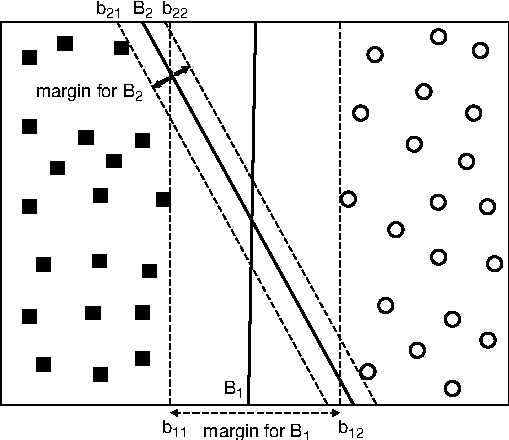
\includegraphics[width=0.5\textwidth]{Images/svm-hyperplanes.pdf}
    \caption[Maximum Margin Hyperplanes]{Maximum Margin Hyperplanes. Tomado de \cite{tan2005introduction}.}
    \label{fig:svm-hyperplanes}
  \end{figure}
\end{frame}

\subsection{\textsc{Self-organizing Maps (SOM)}}
\begin{frame}{\textsc{Self-organizing Maps (SOM)}}
  Es un mapa discreto de $o$ neuronas con vectores $\vw \in \R^m$ que se adaptan a una entrada de $\mX \in \R^{m \times N}$ de $N$ patrones. Tiene una adaptación con una tasa de aprendizaje $\alpha_t$ y un área de afectación $\sigma_t$ que se reducen por cada iteración $t \in \{0, \ldots, T\}$.
  \begin{figure}
    \centering
    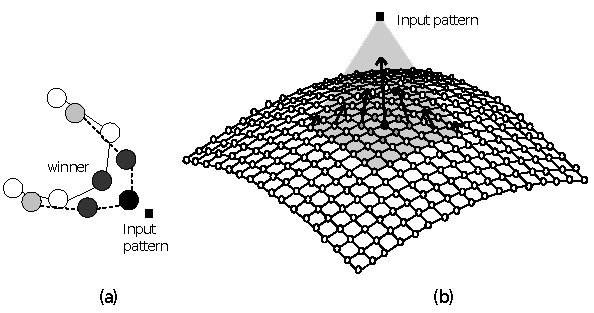
\includegraphics[width=0.75\textwidth]{Images/som-adaptive-proc.pdf}
    \caption[Proceso de adaptación de \textsc{SOM}]{Proceso de adaptación de \textsc{SOM}, (a)~uni--dimensional, (b)~bi--dimensional. Tomado de \cite{de2006fundamentals}.}
    \label{fig:som-adap-proc}
  \end{figure}
\end{frame}

% \begin{frame}{Ejemplo de \textsc{SOM}}
%   \begin{figure}
%     \centering
%     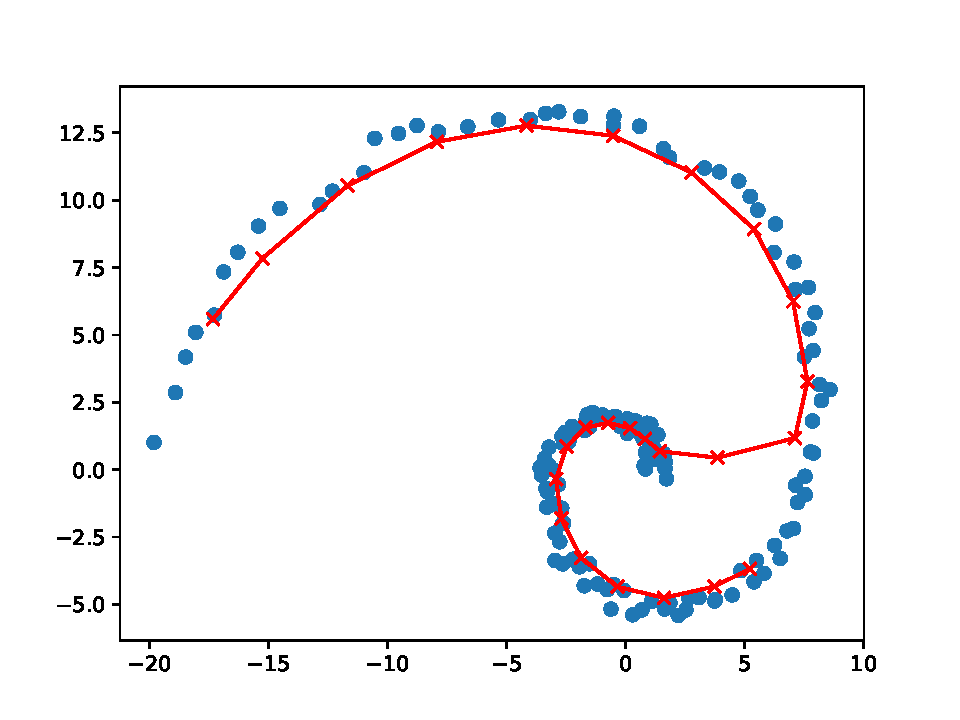
\includegraphics[width=0.75\textwidth]{Images/som-implementation-example25.pdf}
%     \caption[Ejemplo de salida de \textsc{som} uni-dimensional]{Ejemplo de salida de \textsc{som} uni-dimensional con 25 neuronas. Implementación propia.}
%     \label{fig:som-impl-example}
%   \end{figure}
% \end{frame}

\begin{frame}{Aplicación de \textsc{SOM} en perfilamiento de criminales}
  \begin{figure}
    \centering
    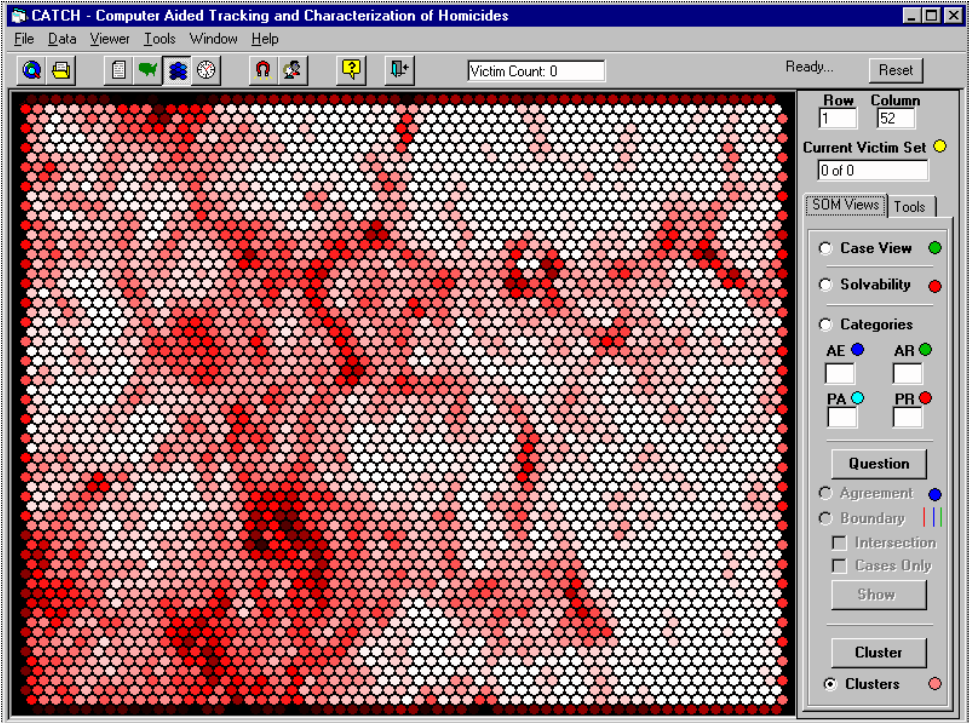
\includegraphics[width=0.75\textwidth]{Images/som-example.png}
    \caption[Ejemplo de uso de \textsc{SOM} en aplicaciones de perfilado]{Ejemplo de uso de \textsc{SOM} en aplicaciones de perfilado. Tomado de \cite{mena2003investigative}.}
    \label{fig:som-example}
  \end{figure}
\end{frame}

% ================================================================

\section{Problemas y soluciones}

\subsection{\textsc{Modelo 1:} Predicción de etiquetas de Twitter}

\begin{frame}{\textsc{Modelo 1:} Problema}
  \begin{alertblock}{Tweet}
    \begin{quote}
    ``Really excited to add @plaidavenger to my \textbf{\#deathlist} along with Italy and @Plaid\_Obama after receiving that information. \textbf{\#KillEveryone} \textbf{\#ISIS}''
    \end{quote}
  \end{alertblock}
\end{frame}

\begin{frame}{\textsc{Modelo 1:} Predicción de etiquetas de Twitter}
  \begin{alertblock}{?`Que hacer?}
    Con un modelo de regresión lineal predecir los hashtags de los tweets.
  \end{alertblock}
  \vspace{2em}
  
  \begin{tabular}{p{0.47\textwidth} p{0.05\textwidth} p{0.46\textwidth}}
    ``Really excited to add @plaidavenger to my deathlist along with Italy and @Plaid\_Obama after receiving that information.'' & $\mathlarger{\mathlarger{\mathlarger{\Rightarrow}}}$ & \textbf{\#deathlist, \#KillEveryone, \#ISIS}
    \end{tabular}
\end{frame}

\begin{frame}{Representación de palabras: \textsc{Bag of Words}}
  $N$ es el tamaño del diccionario de términos $D$ (e.g. $N = |D|$).
  \begin{equation*} \label{eq:bow-repr1}
    \text{word2idx} = \Big\{(t_i, i) : \forall i \in \{1, \ldots, N\} \Big\}
  \end{equation*}
  
  \begin{equation*} \label{eq:bow-repr2}
    \text{idx2word} = \Big[t_1, \ldots, t_N\Big]
  \end{equation*}

  \begin{alertblock}{Representación de palabras en vectores para \textsc{BoW}}
    Para un termino individual su vector representativo se define como:
    \begin{equation*}
      \ve^{(i)} = [0, \ldots, 1, \ldots, 0] \leftarrow \text{posicion } i\text{--\'esima}
    \end{equation*}
    \begin{equation*}
      \ve^{(i)}, (t, i) \in \text{word2idx}
    \end{equation*}
    Para un documento $d$ de términos, se calcula por cada termino que existen dentro del diccionario su vector representativo como:
    \begin{equation*} \label{eq:bow-word-vector-sum}
      \vs = \mathlarger{\mathlarger{\sum}}_{(t, i) \in \text{word2idx}} \ve^{(i)}, t \in d
    \end{equation*}
  \end{alertblock}
\end{frame}

\begin{frame}{Representación de palabras: \textsc{TF--IDF}}
  \textsc{TF--IDF} $=$ Term Frequency -- Inverse Document Frequency
  \begin{alertblock}{Propósito}
    Darle mayor importancia a las palabras que ocurren con frecuencia intermedia en el documento $d$ y en el corpus $D$.
  \end{alertblock}
  \begin{equation*} \label{eq:tf-repr}
    \text{tf}(t,d) = \text{Frecuencia del termino (o n--grama) } t \text{ en el documento } d
  \end{equation*}

  \begin{equation*} \label{eq:idf-repr}
    \text{idf}(t, D) = \text{log}\Bigg( \frac{N}{|\{d \in D : t \in d\}|} \Bigg) ; N = |D|
  \end{equation*}

  \begin{equation*} \label{eq:tfidf-repr}
    \text{tf-idf}(t, d, D) = \text{tf}(t, d) \cdot \text{idf}(t, D)
  \end{equation*}
\end{frame}

\begin{frame}{Regresión lineal}
  Para una vector de parámetros $\vtheta$ y un vector de características $\vx$, la regresión lineal se puede definir como:
  \begin{equation*}
    \hat{y}(\vx, \vtheta) = \vtheta^{\top} \vx = \theta_0 + \theta_1 x_1 + \cdots + \theta_n x_n
  \end{equation*}

  Donde $\hat{y}(\vx, \vtheta) \,:\, \R^n \times \R^n \rightarrow \R$.
  
  $\theta_0$ se le conoce como el \emph{bias} del modelo.

  El objetivo es que para una salida esperada $y$ se tenga la salida $\hat{y}$ con menor error por medio de ajustar los valores de $\vtheta$. De forma que se quiere:
  \begin{equation*}
    \vtheta = \text{arg m\'{\i}n}_{\vtheta} | \hat{y}(\vx, \vtheta) - y|
  \end{equation*}

\end{frame}

\begin{frame}{Regresión logística $\sigma(x)$}
  \noindent\begin{minipage}{0.6\textwidth}
    \begin{figure}[H]
      \centering
      \begin{tikzpicture}[scale=0.80]
        \begin{axis}[ 
          xlabel=$x$,
          ylabel={$\sigmoid(x)$}
          ] 
          \addplot {1 / (1+exp(-x))}; 
        \end{axis}
      \end{tikzpicture}
      \caption[Gráfica de función sigmoide]{Gráfica de función sigmoide.}
      \label{fig:logits-example}
    \end{figure}
  \end{minipage}%
  \hfill%
  \begin{minipage}{0.35\textwidth}
    \begin{equation*}
      \sigmoid(x) = \frac{1}{1+\exp(-x)}
    \end{equation*}
    
    \begin{equation*}
      \sigmoid(x) \,:\, \R \rightarrow (0,1)
    \end{equation*}
    Evita problemas de \textsc{Bias} y \textsc{Overfitting} del modelo
  \end{minipage}
\end{frame}

\begin{frame}{One vs Rest}
  \noindent\begin{minipage}{0.5\textwidth}
    \begin{figure}[H]
      \centering
      % \missingfigure{Hacer la arquitectura en yEd}
      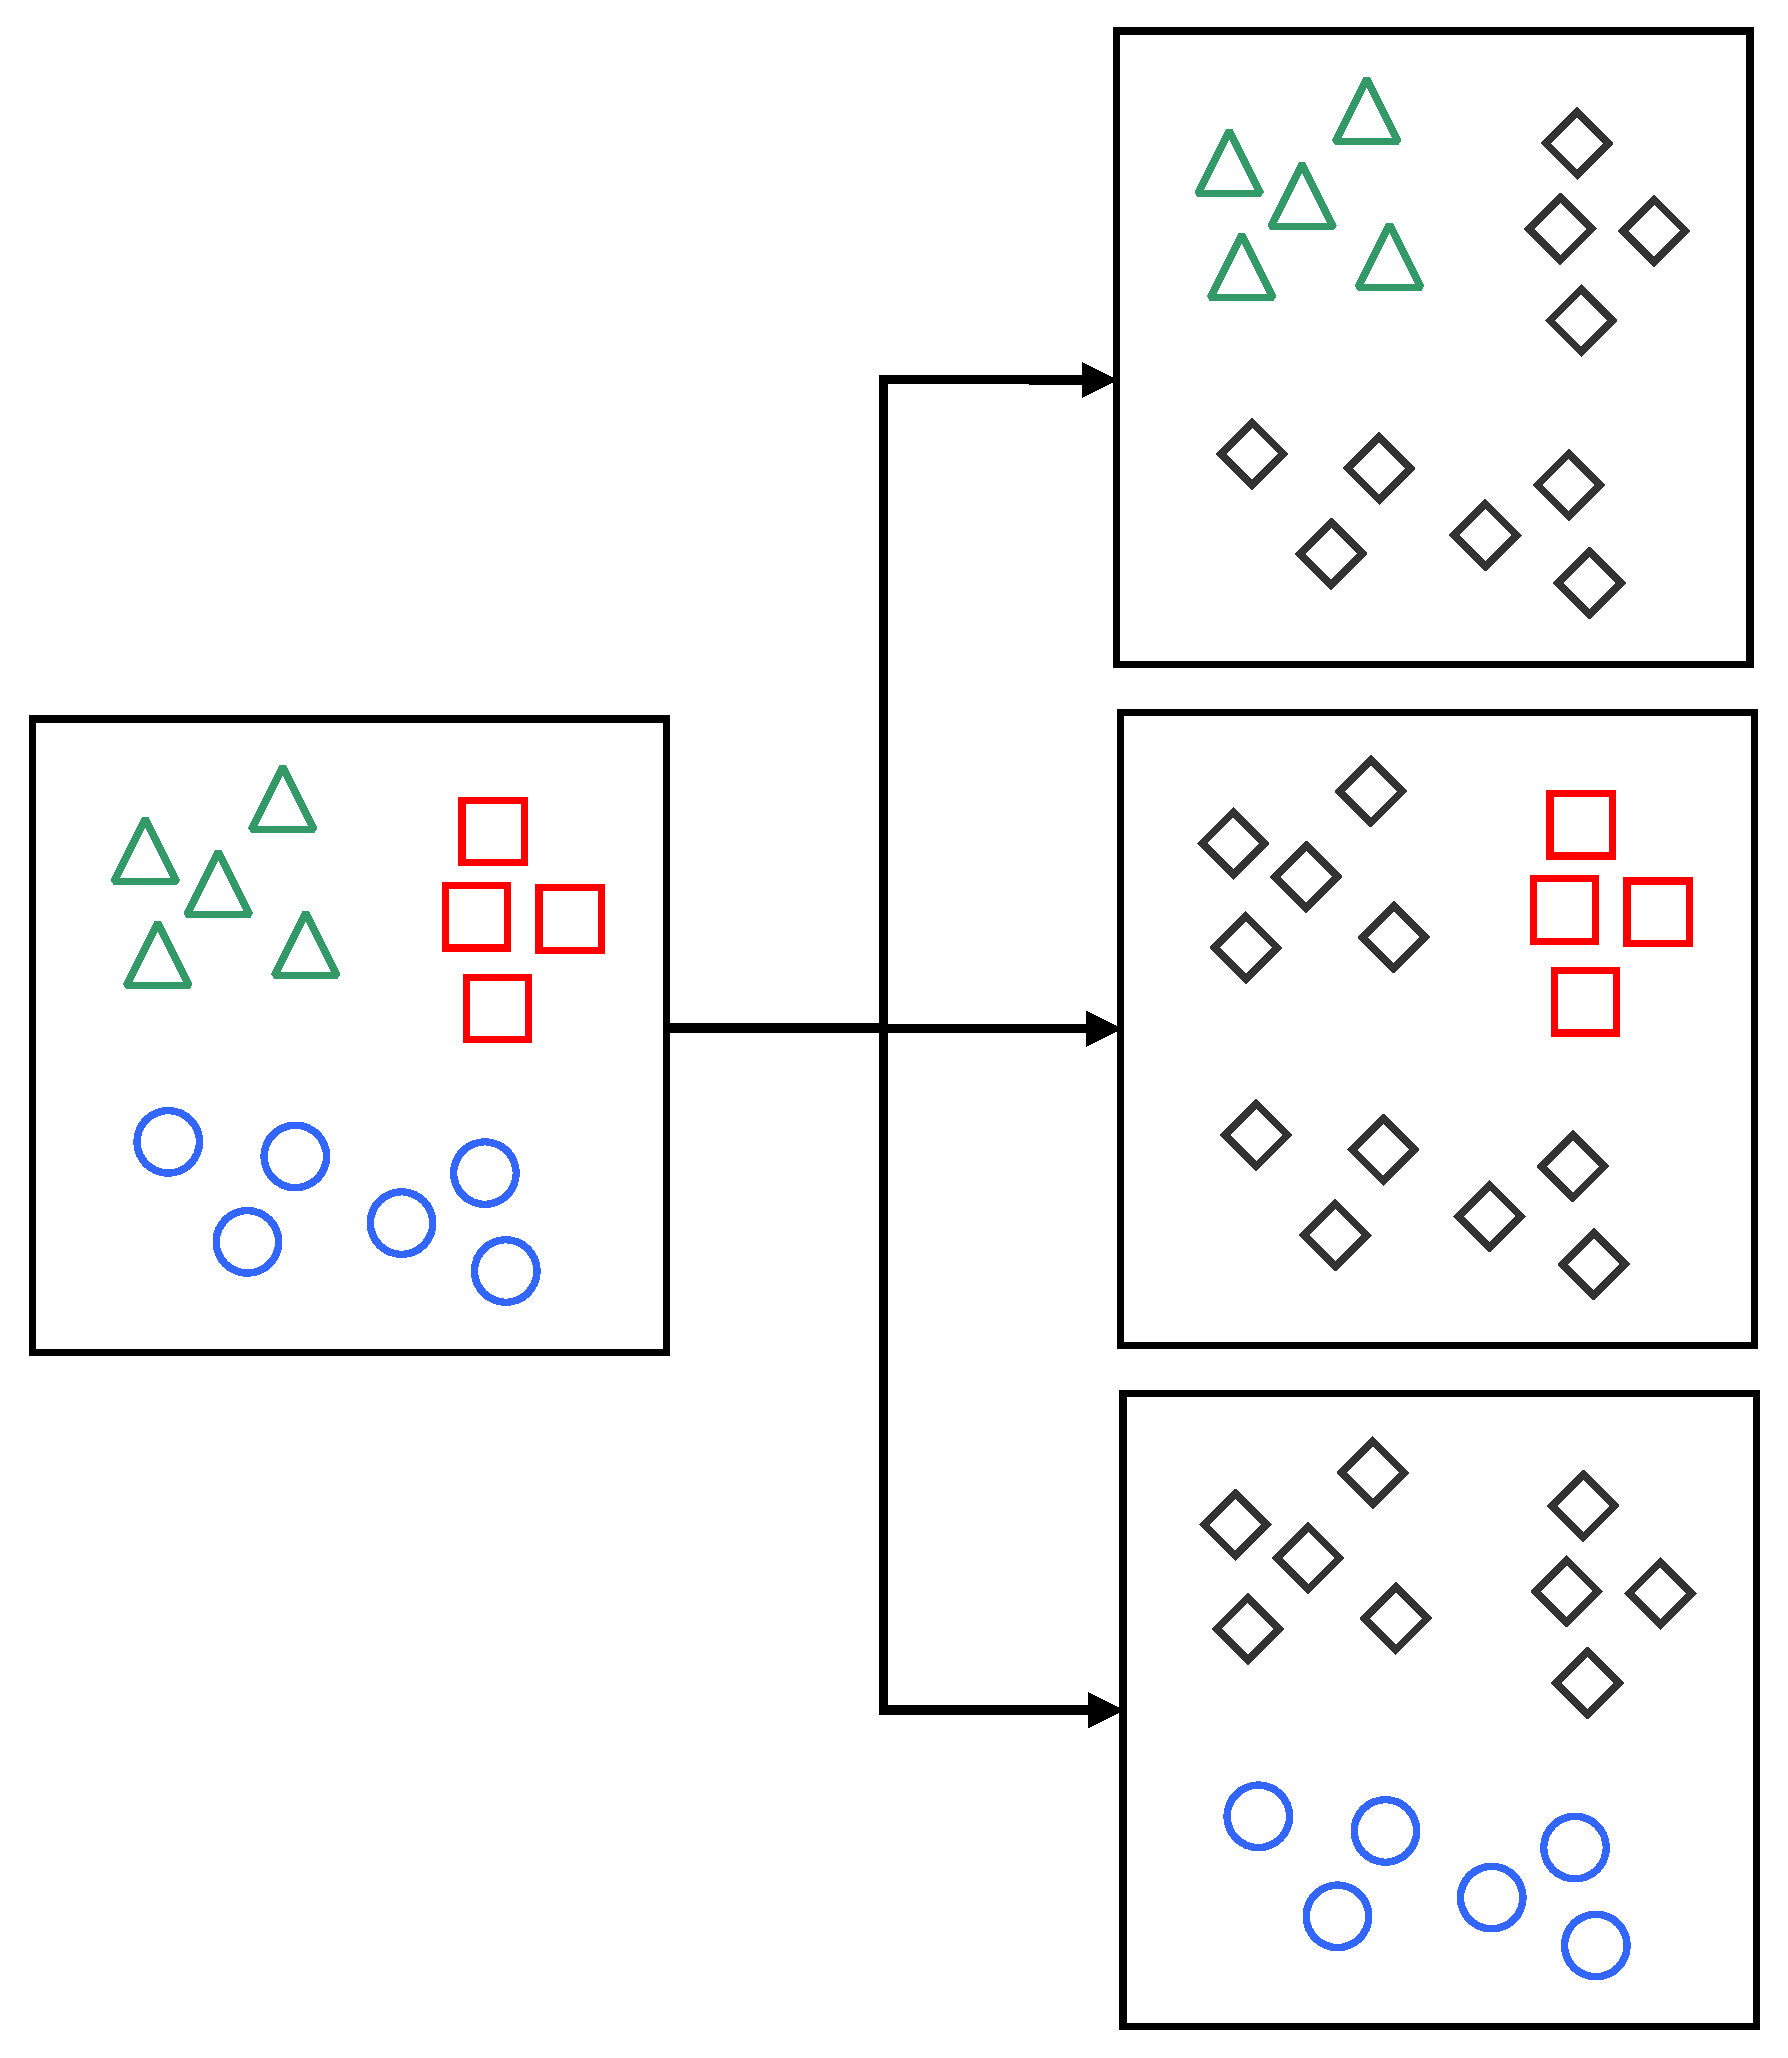
\includegraphics[width=\textwidth]{Images/one-vs-rest.pdf}
      \caption[Algoritmo de One vs Rest]{Algoritmo de One vs Rest.}
      \label{fig:ovr-algo}
    \end{figure}
  \end{minipage}%
  \hfill%
  \begin{minipage}{0.45\textwidth}
    Se entrenan $C$ estimadores $\vtheta_i$ para cada clase con algún algoritmo de optimización (ej. gradiente descendiente). \\
    
    Se determina un estimador $c \in \{1, \ldots ,C\}$, que se calcula como:
    \begin{equation*}
      c = \text{arg max}_i \, \sigmoid(\vtheta_i^{\top} \vx)
    \end{equation*}
  \end{minipage}
\end{frame}

\begin{frame}{Predicción de hashtags}
  A partir de un diccionario previamente definido a entrenar el \textsc{One vs Rest} de forma:
  \begin{equation*}
    \{(i, h)\} \,;\, h \in \text{hashtags} \,;\, i \in \{1, \ldots, C\}
  \end{equation*}

  De forma que se recupera el hashtag $h$ correspondiente a partir de la clase estimada $i$ por \textsc{One vs Rest}.
\end{frame}

\subsection{\textsc{Modelo 2:} Reconocimiento de \textsc{Named Entities} con redes \textsc{LSTM}}

\begin{frame}{\textsc{Modelo 2:} Problema}
  \alert{?`De que y de quienes están hablando?}
  
\begin{alertblock}{Tweet: @realDonaldTrump}
  \begin{quote}
    ``The \textbf{Democrats} new and pathetically untrue sound bite is that we are in a “Constitutional Crisis.” They and their partner, the \textbf{Fake News Media}, are all told to say this as loud and as often as possible. They are a sad JOKE! We may have the strongest \textbf{Economy} in our history, best ...''
  \end{quote}
\end{alertblock}
\end{frame}

\begin{frame}{\textsc{Modelo 2:} Reconocimiento de \textsc{Named Entities} con redes \textsc{LSTM}}
  Son redes neuronales recurrentes que son capaces de reconocer \textsc{Named Entities}.
  \begin{table}
    \centering
    \begin{tabular}{l|lllllll} 
      \textbf{Texto}    & Donald   & Trump & es & presidente & de & Estados & Unidos \\
      \textbf{Etiqueta} & B-PER    & I-PER & O  & O          & O  & B-ORG   & I-ORG
    \end{tabular}
    \\ [1em]
    \caption{Ejemplo de reconocimiento de \textsc{Named Entities}.}
    \label{table:namedent-example}
  \end{table}

  \begin{table}
    \centering
    \begin{tabular}{rl} 
      Otro & O \\
      Persona & PER \\
      Ubicación & LOC \\
      Organización & ORG \\
      Misceláneo & MISC \\
    \end{tabular}
    \caption{Categorías de \textsc{Named Entities}.}
    \label{table:namedent-categories}
  \end{table}
\end{frame}

\begin{frame}{Redes neuronales recurrentes (\textsc{RNN})}
  \begin{figure}[H]
    \centering
    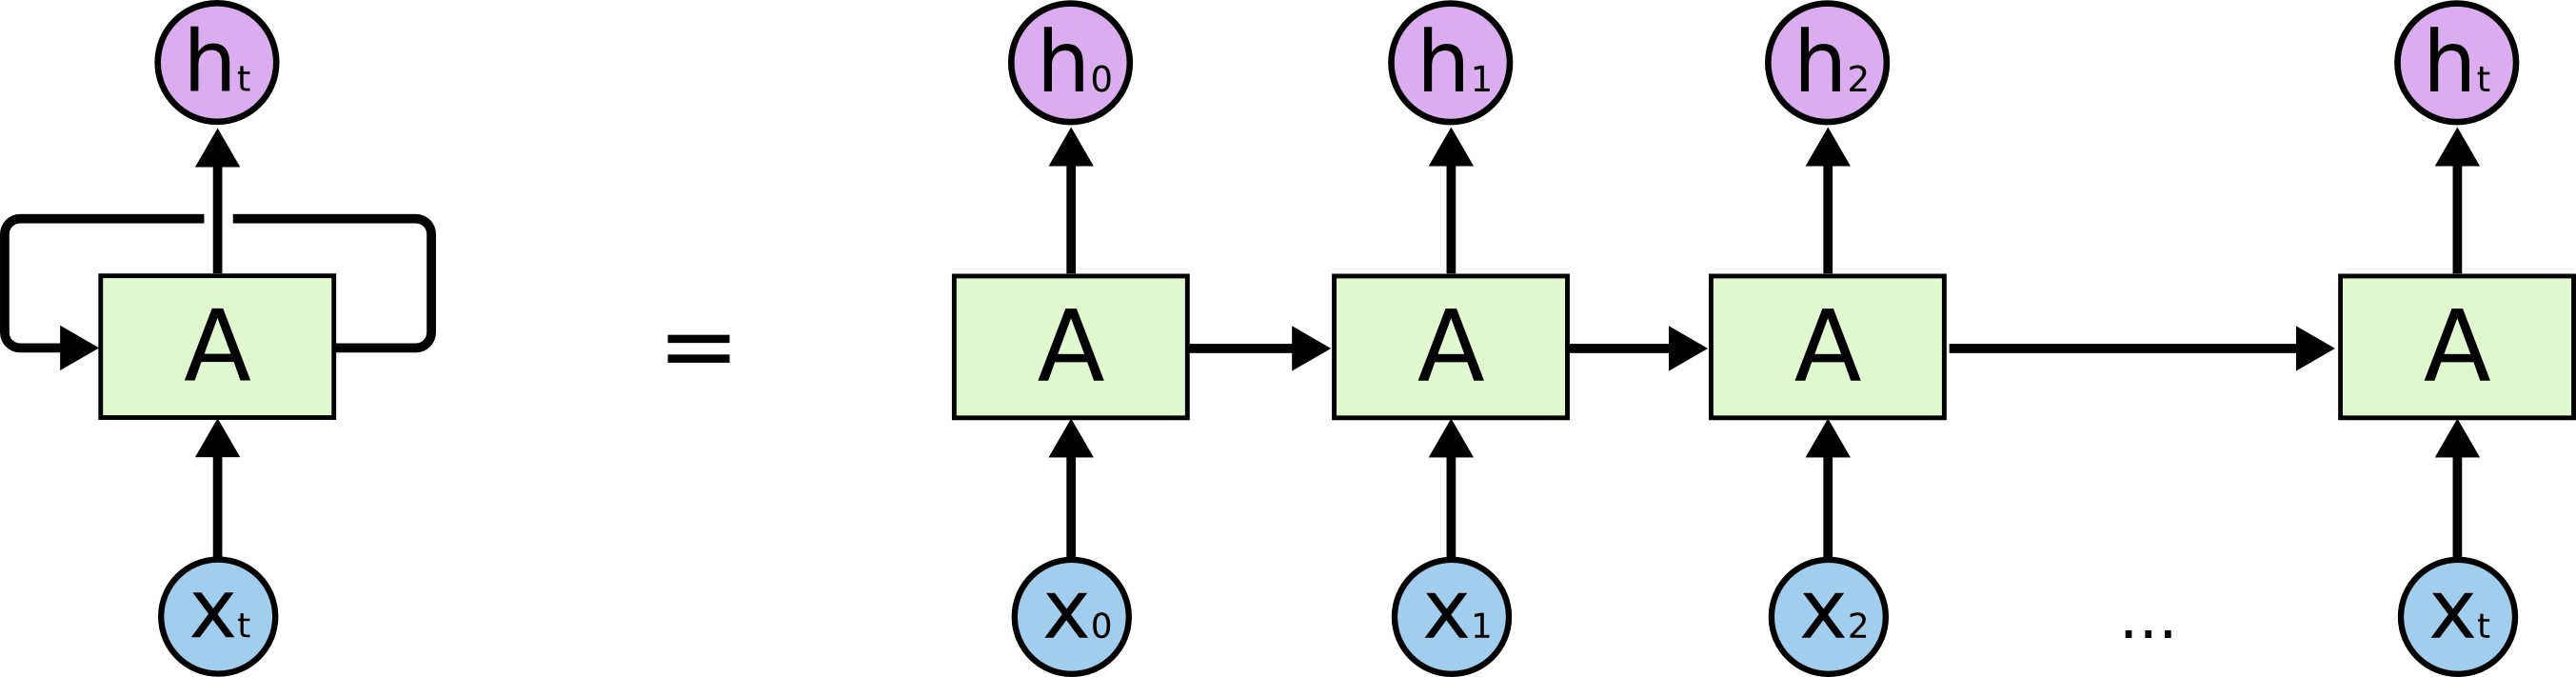
\includegraphics[width=0.6\textwidth]{Images/RNN-unrolled.png}
    \caption[Red \textsc{RNN} simplificada]{Red \textsc{RNN} simplificada. Tomado de \cite{understanding-lstm}.}
    \label{fig:rnn-classic-simple}
  \end{figure}

  \begin{figure}[H]
    \centering
    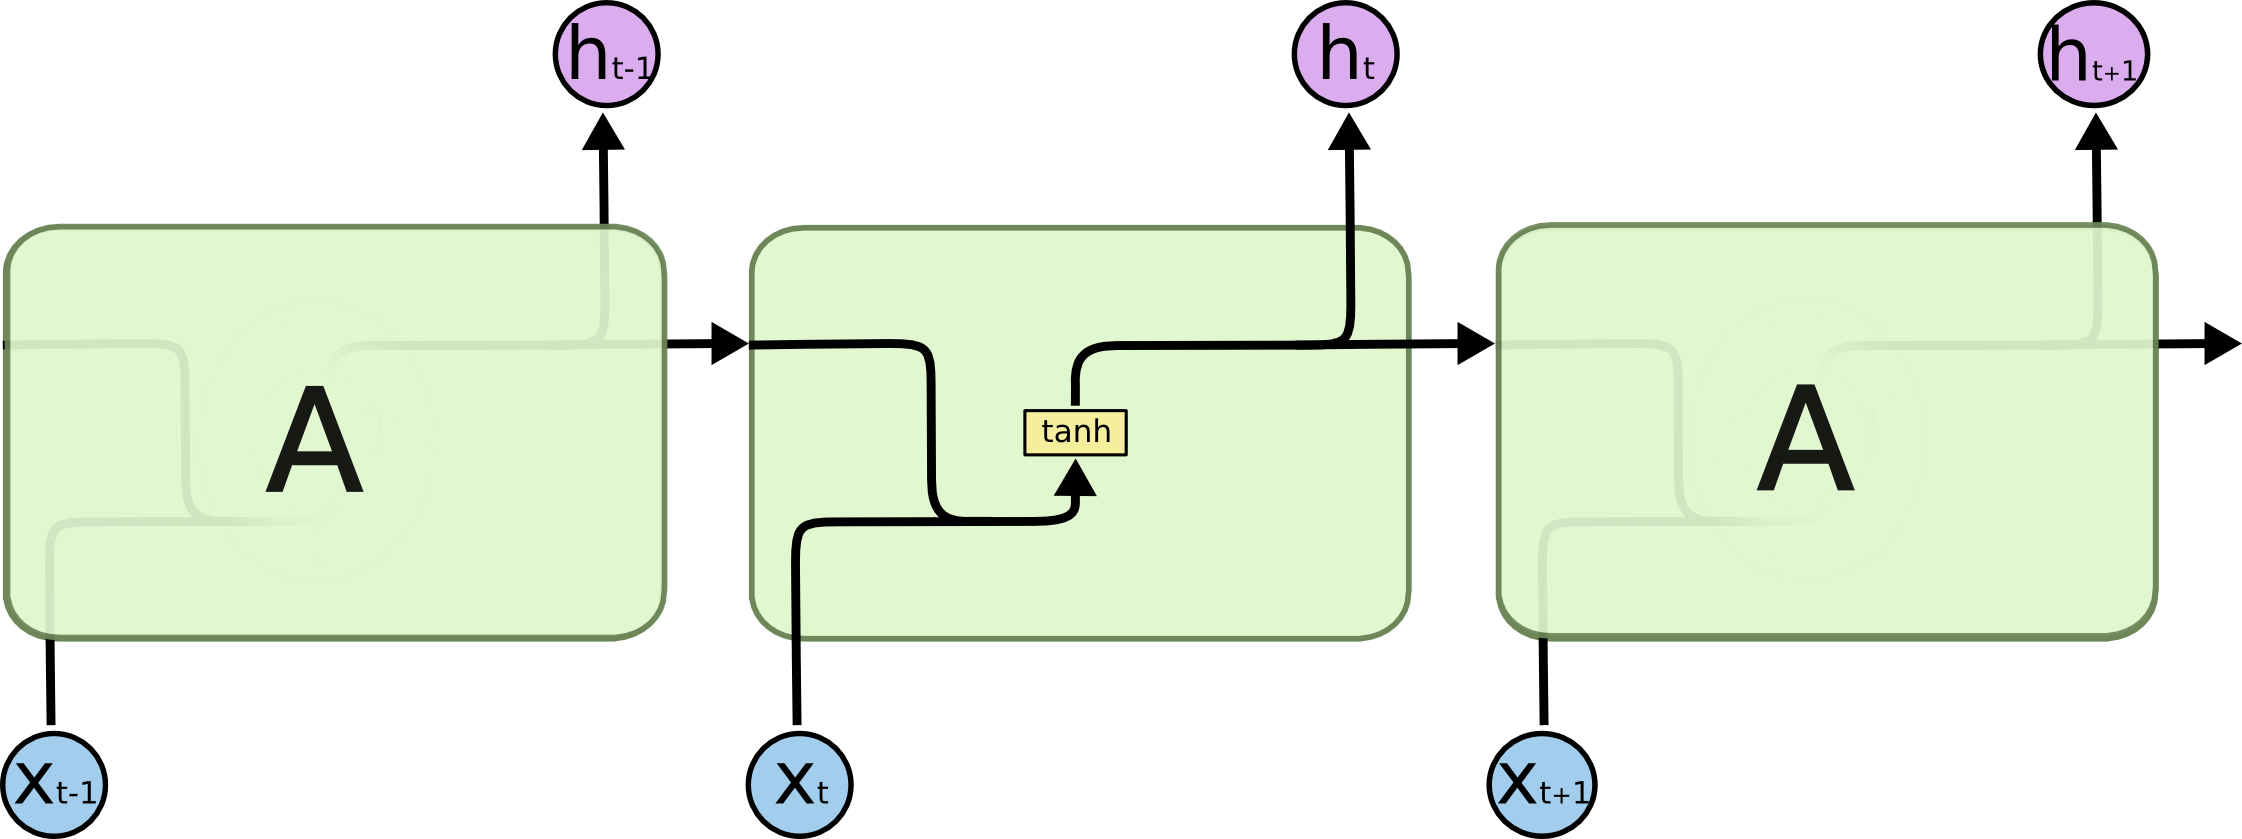
\includegraphics[width=0.6\textwidth]{Images/LSTM3-SimpleRNN.png}
    \caption[Arquitectura \textsc{RNN} clásica]{Arquitectura \textsc{RNN} clásica. Tomado de \cite{understanding-lstm}.}
    \label{fig:rnn-classic}
  \end{figure}
\end{frame}

\begin{frame}{Redes \textsc{Long Short Term Memory (LSTM)}}
  \begin{figure}[H]
    \centering
    % \missingfigure{Hacer la arquitectura en yEd}
    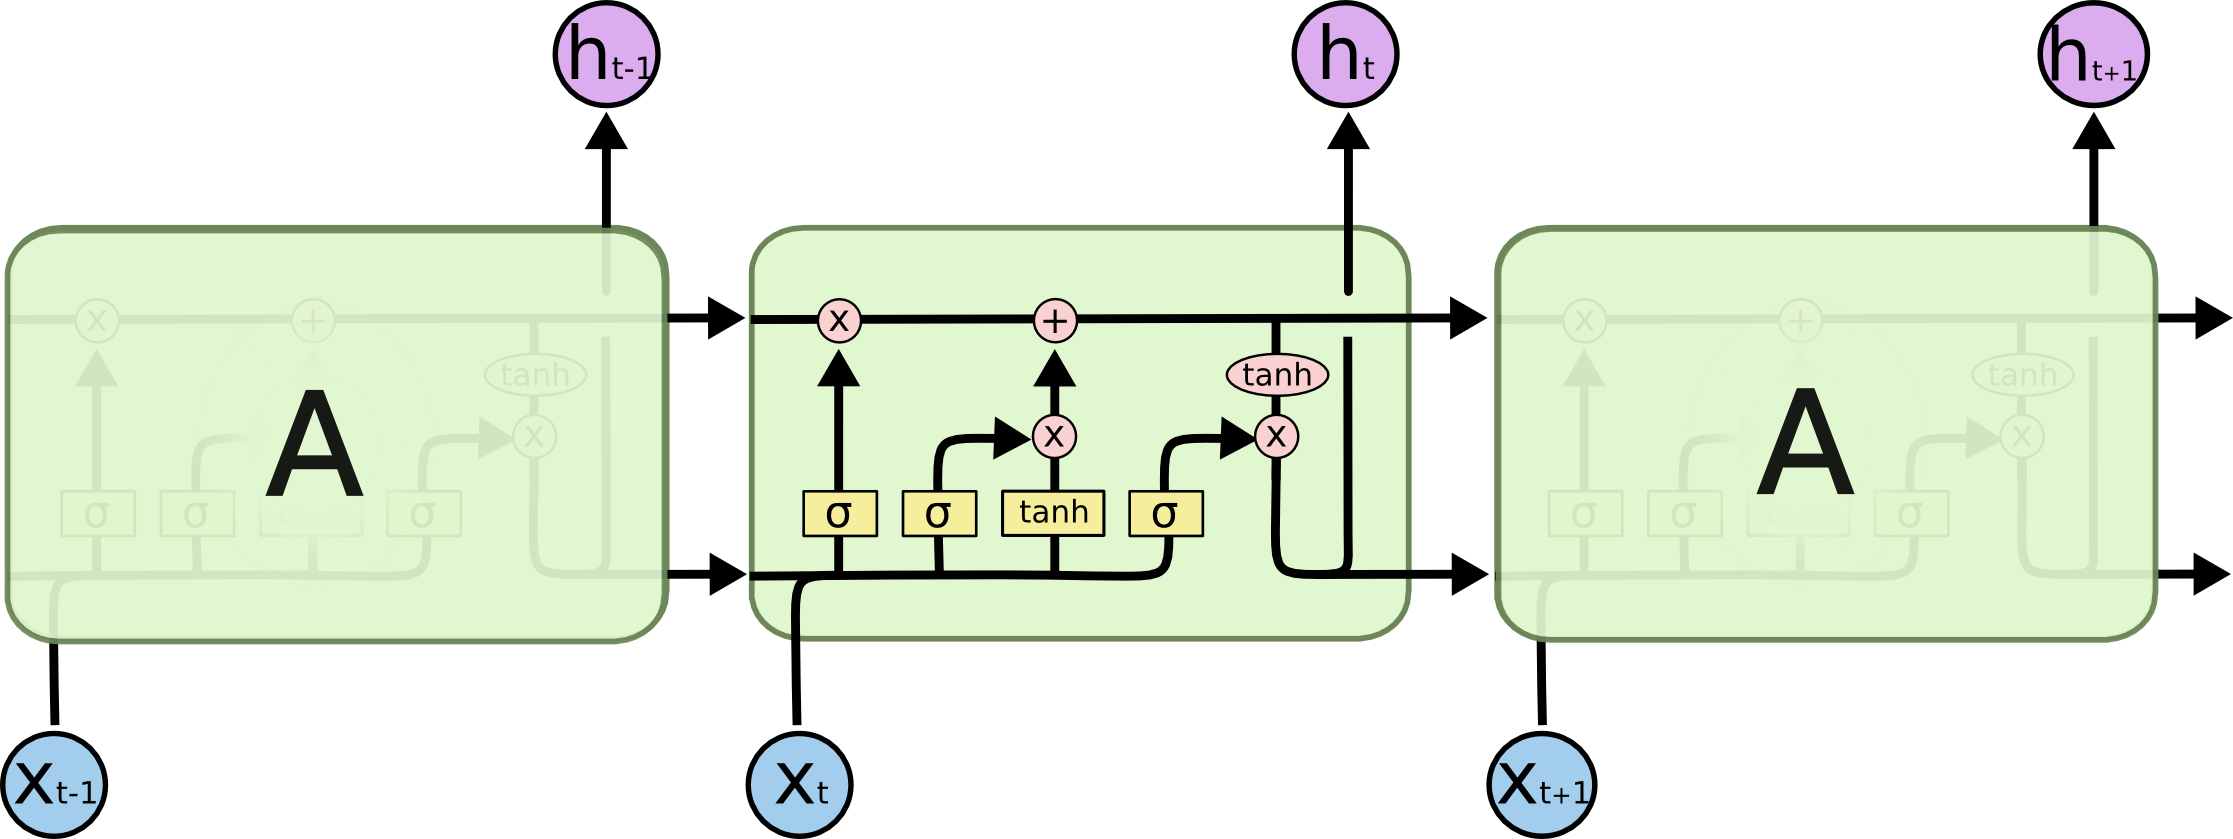
\includegraphics[width=0.9\textwidth]{Images/LSTM3-chain.png}
    \caption[Arquitectura de red \textsc{LSTM} clásica]{Arquitectura de red \textsc{LSTM} clásica. Tomado de \cite{understanding-lstm}.}
    \label{fig:lstm-classic}
  \end{figure}

  \begin{alertblock}{Nota}
    Estas redes son solo \emph{feedforward} (e.g. hacia adelante). Solo se basan en entradas pasadas.
  \end{alertblock}
\end{frame}

\begin{frame}{Redes \textsc{Bidirectional Long Short Term Memory (Bi-LSTM)}}
  \begin{figure}[H]
    \centering
    % \missingfigure{Hacer la arquitectura en yEd}
    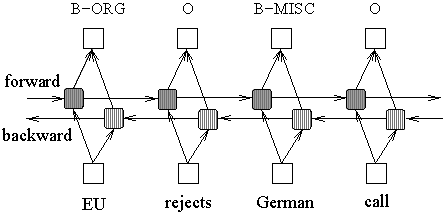
\includegraphics[width=0.6\textwidth]{Images/bilstm-arch.pdf}
    \caption[Etiquetado con una \textsc{Bi-LSTM}]{Etiquetado con una \textsc{Bi-LSTM}. Tomado de \cite{Huang2015}.}
    \label{fig:bilstm-arch}
  \end{figure}

  \begin{alertblock}{Nota}
    Estas redes son \emph{feedforward} como \emph{backward}. Se basan de entradas pasadas y futuras.
  \end{alertblock}
\end{frame}


% \begin{frame}{Entrenamiento y uso de redes \textsc{Bi-LSTM}}
%   Se procede primeramente por entrenar el modelo con un dataset, que establece la relación $(t, e)$ de las palabras $t$ y las \emph{Entities} $e$.

%   Las librerías en uso son \textsc{TensorFlow} y \textsc{Numpy}.
% \end{frame}

\subsection{\textsc{Modelo 3:} Búsqueda de tweets relacionados con \emph{embeddings}}

\begin{frame}{?`Que son los \emph{embeddings}?}
  Son espacios de vectores $n$--dimensionales que se mapean según una palabra.

  Tómese $\vp_{t}$ como el vector que representa el termino $t$ y a $d$ como la distancia calculada entre los vectores (típicamente la distancia \textbf{coseno}).

  \begin{alertblock}{Ejemplo}
    $d(\vp_{\text{asombroso}}, \vp_{\text{genial}})$ debería tener un valor bajo.
    
    $d(\vp_{\text{asombroso}}, \vp_{\text{terrible}})$ debería tener un valor alto.
  \end{alertblock}

  También se pueden representar varias palabras de un documento en un solo vector por medio de sumarlos. (i.e. $\sum_{t \in d}\vp_{t}$).
\end{frame}

\begin{frame}{\textsc{Modelo 3:} Búsqueda de tweets relacionados con \emph{embeddings}}
  Es posible categorizar los $k$ textos mas parecidos a una consulta $q$ en base a su embedding con otros textos recopilados.

  \begin{alertblock}{StarSpace}
    Genera embeddings en base a un dataset de entrenamiento. Desarrollado por Facebook Research en 2017 \cite{starspace}. 
  \end{alertblock}
\end{frame}

\section{Conclusiones y trabajo futuro}

\begin{frame}{Conclusiones}
  \begin{itemize}
  \item Se investigaron diferentes metodologías de NLP y Data Science para la tarea de perfilado de cibercriminales por medio de informacion de fuentes abiertas.
  \item Es necesario probar las metodologías propuestas con información obtenida de fuentes abiertas que este validada de forma que el entrenamiento de ellos sean efectivos en la tarea.
  \end{itemize}
\end{frame}

\begin{frame}{Trabajo futuro}
  \begin{itemize}
  \item Implementación de los modelos 2 y 3 propuestos con propósito de ayudar al perfilamiento de cibercriminales.
  \item Recopilar datos pertinentes para el entrenamiento de los modelos propuestos.
  \item Adaptar y generalizar los modelos para el uso del lenguaje español.
  \item Implementar un modelo de recolección de información de redes sociales de cibercriminales de forma que sea mas fácil perfilarlos contra futuros.
  \item Realizar una visualización en dashboard de los algoritmos propuestos para ayudar al agente a realizar el perfilamiento.
  \end{itemize}
\end{frame}

\appendix
\setbeamertemplate{bibliography item}{\insertbiblabel}
\begin{frame}[allowframebreaks]{Bibliografía}

  % \nocite{*}
  \bibliography{demo}
  \bibliographystyle{abbrv}

\end{frame}

\end{document}
